\documentclass{beamer}
\usepackage[utf8]{inputenc}
\usetheme{Madrid}
\usecolortheme{beaver}
\usepackage{amsmath,amsfonts,amsthm,bm} % Math packages
\usepackage{hyperref}
%\usepackage{makecell}
%Information to be included in the title page:
\title{Vector Auto Regressions in macroeconomics}
\author{Daniele Caratelli}
\institute{Stanford University}
\date{\today}



\begin{document}
	\newcommand{\semitransp}[2][35]{\color{fg!#1}#2}
	\frame{\titlepage}
	
	\begin{frame}{Chocolate!}
		\begin{figure}
		\centering
		\includegraphics[width=0.7\linewidth]{figures/Chocolate}
		\end{figure}

	\end{frame}
	
	\begin{frame}
		\frametitle{Disclaimer}
		The views expressed here are those of the author and the author alone. They do not reflect those of Profs. Tom MaCurdy and Frank Wolak or those of Stanford University more broadly.	
	\end{frame}
	
	\begin{frame}{Macroeconomic data}
	\begin{figure}
		\centering
		\includegraphics[width=0.7\linewidth]{figures/fig3}\\
		\includegraphics[width=1\linewidth]{figures/Header}
		\caption{(Some) macro data by category}
		\label{fig:fig3}
	\end{figure}
	\end{frame}

	\begin{frame}{Macroeconomic data, cnt'd}
		\begin{itemize}
			\item lots of data
			\item move along the \textit{business cycle}
			\item idiosyncratic (leads and lags)
		\end{itemize}
			\pause
			\vspace*{1em}				
			\underline{Uses}:
			\begin{itemize}
				\item[1.] Forecasting
				\item[2.] Data description
				\item[3.] Structural inference
				\item[4.] Policy analysis
			\end{itemize}
			\pause
			\vspace*{1em}
		$\Rightarrow$ want statistical model to deal with macroeconomic variables.			
	\end{frame}
	
	\begin{frame}{A brief history}
		\hfill\begin{minipage}{\dimexpr\textwidth-0.5cm}
			\only<1>{\begin{itemize}
			\item Collecting macroeconomic data (e.g. NIPA) \hfill '30s-'40s
			\item Large-scale models \hfill  '60s-present
			\item VARs \hfill '70s-present
			\item DFMs \hfill '80s-present
			\item Nowcasting \hfill '00s-present
			\end{itemize}}
			\only<2>{\begin{itemize}
			\vspace*{.85em} 
			\item Large-scale models \hfill  '60s-'80s
			\begin{itemize}
			\item[$\times$] many equations informed by macro theory,
			\item[$\times$] each with just a few variables, mostly considered exogenous,
			\item[$\times$] problem: hard to discover empirical facts.
			\end{itemize}
			\end{itemize}}
			\only<3>{\begin{itemize}
			\vspace*{2.5em}
			\item VARs \hfill '70s-present
			\begin{itemize}
				\item[$\times$] let the data speak (under identification assumptions),
				\item[$\times$] consistent with rational expectations.
			\end{itemize}
			\end{itemize}}
		\end{minipage}
	\end{frame}
	
	
	\begin{frame}
		\frametitle{From AR to V-AR}
		An AR(p) process for $y$ is:
		$$y_{t} = \mu +\rho_{1}y_{t-1} + \dots \rho_{p} y_{t-p} + \varepsilon_{t}, \hspace{1em} \varepsilon_{t}\sim \mathcal{N}(0,\sigma^{2})$$
		\pause
		What if we are interested in $n$-many variables each having an AR(p) process?
		\pause
		(1) holds for each of these and so:
		$$\begin{cases}
		y_{1t} = \mu_{1} +\rho_{1}^{1}y_{1t-1} + \dots \rho_{p}^{1} y_{1t-p} + \varepsilon_{1t},\\
		\vdots \\
		y_{nt} = \mu_{n} +\rho_{1}^{n}y_{nt-1} + \dots \rho_{p}^{n} y_{1t-p} + \varepsilon_{nt},
		\end{cases}$$
		with $\varepsilon_{it}\sim \mathcal{N}(0,\sigma_{i}^{2})$.		
	\end{frame}
	
	\begin{frame}
		\frametitle{From AR to V-AR, cnt'd}
		Stack!!
		\begin{center}
			$$\underbrace{\begin{bmatrix}
				y_{1t}\\
				\vdots\\
				y_{nt}
			\end{bmatrix}}_{\bm{Y_{t}}} = \underbrace{\begin{bmatrix}
			\mu_{1}\\
			\vdots\\
			\mu_{n}
			\end{bmatrix}}_{\bm{\mu}} + \Phi_{1}\times \underbrace{\begin{bmatrix}
			y_{1t-1}\\
			\vdots\\
			y_{nt-1}
			\end{bmatrix}}_{\bm{Y_{t-1}}}\dots  + \Phi_{p} \times \underbrace{\begin{bmatrix}
			y_{1t-p}\\
			\vdots\\
			y_{nt-p}
			\end{bmatrix}}_{\bm{Y_{t-p}}} + \underbrace{\begin{bmatrix}
			\varepsilon_{1t}\\
			\vdots\\
			\varepsilon_{nt}
			\end{bmatrix}}_{\bm{\varepsilon_{t}}}$$ 
		where 
		$$\Phi_{i} = \begin{bmatrix}
		\rho_{i}^{1} & \dots & \dots & 0\\
		0 & \rho_{i}^{2} & \dots & 0 \\		
		\dots & \dots & \ddots & \dots\\
		0 & \dots & \dots & \rho_{i}^{n}\\			
		\end{bmatrix} \hspace{4em} \bm{\varepsilon}\sim \sigma^{2}I_{n\times n}$$
		\end{center}	
	\end{frame}	
	
	\begin{frame}[label=system]{VAR(p)}
		As (macroeconomic) variables are all ``connected" we can extend the above so that each variable depends not only on its own lags but also on the lags of the other variables.\\
		Then we have the following system:
		\only<1>{$$\small{\begin{cases}
		y_{1t} = \mu_{1} +\rho_{11}^{1}y_{1t-1} + \dots \rho_{1p}^{1} y_{1t-p} + \dots + \rho_{1n}^{1}y_{nt-1} + \dots \rho_{pn}^{1} y_{nt-p} +\varepsilon_{1t},\\
		\vdots \\
		y_{nt} = \mu_{n} +\rho_{11}^{n}y_{1t-1} + \dots \rho_{1p}^{n} y_{1t-p} + \dots + \rho_{1n}^{n}y_{nt-1} + \dots \rho_{pn}^{n} y_{nt-p} +\varepsilon_{nt},\\
		\end{cases}}$$
		\vfill
		
		\hyperlink{chol}{\beamergotobutton{Chol}}}
		\pause
		\only<2,3>{$$\bm{Y_{t}} = \bm{\mu} + \Phi_{1} \bm{Y_{t-1}} + \dots \Phi_{p}\bm{Y_{t-p}} + \bm{\varepsilon_{t}}$$}
		\pause
		$$\Phi_{i} = \begin{bmatrix}
		\rho_{i1}^{1} & \rho_{i2}^{1} & \cdot & \rho_{in}^{1}\\
		\cdot & \cdot & \cdot &\cdot\\
		\rho_{i1}^{n} & \rho_{i2}^{n} & \cdot & \rho_{in}^{n}\\				
		\end{bmatrix}$$
	\end{frame}
	
	\begin{frame}{VAR, OLS formulation}
		Finally, we can can stack once again and write the VAR(p) as a VAR(1):
		$$\underbrace{\begin{bmatrix}
		\bm{Y_{t}}\\
		\bm{Y_{t-1}}\\
		\vdots\\
		\bm{Y_{t-(p-1)}}
		\end{bmatrix}}_{np\times 1} = \underbrace{\begin{bmatrix}
		\bm{\mu}\\
		\bm{\mu}\\
		\vdots\\
		\bm{\mu}		
		\end{bmatrix}}_{np\times 1} + \underbrace{\begin{bmatrix}
		\Phi_{1} & \Phi_{2} & \dots & \Phi_{p}\\
		I_{n\times n} & 0_{n\times n} & \dots & 0_{n\times n} \\
		\dots & \ddots & \dots & \dots\\
		0_{n\times n} & \dots & I_{n\times n} & 0_{n\times n} \\		
		\end{bmatrix}}_{np\times np} \underbrace{\begin{bmatrix}
		\bm{Y_{t-1}}\\
		\bm{Y_{t-1}}\\
		\vdots\\
		\bm{Y_{t-p}}
		\end{bmatrix}}_{np\times 1} + \underbrace{\begin{bmatrix}
		\bm{\varepsilon_{t}}\\
		0_{n\times 1}\\
		\vdots\\
		0_{n\times 1}\\		
		\end{bmatrix}}_{np\times 1}$$
		\pause 
		\vspace*{2em}
		$$\bm{\bar{Y}_{t}} = \bm{\bar{\mu}} + \bm{\bar{\Phi}}\bm{\bar{Y}_{t-1}} + \bm{\bar{\varepsilon}_{t}},\footnote{Note this is known as the \textit{companion-form}.} \hspace{2em} \bm{\bar{\varepsilon}}\sim \mathcal{N}(\bm{\bar{0}},\bm{\bar{\Sigma}}),$$
		\pause
		\vspace*{1.5em}
		$\longrightarrow$ run OLS and get $\bm{\bar{\mu}}$ and $\bm{\bar{\Phi}}$ \pause \hfill ($n+pn^{2}$ parameters!)
	\end{frame}
	
%	\begin{frame}{VAR in macroeconomics}
%		\underline{Types}:
%		\begin{itemize}
%			\item Reduced-form
%			\item Recursive \hspace*{3em}
%			\item Structural
%		\end{itemize}
%	\end{frame}

		
	\begin{frame}{Forecasting}
		\begin{align*}
		E_{t+1}[\bm{\bar{Y}_{t+1}}]&=E_{t+1}[\bm{\bar{\mu}} + \bm{\bar{\Phi}}\bm{\bar{Y}_{t}} + \bm{\bar{\varepsilon}_{t+1}}] =  \bm{\bar{\mu}} + E[\bm{\bar{\Phi}}\bm{\bar{Y}_{t-1}}]\\
		&=\bm{\bar{\mu}} + \bm{\bar{\Phi}}E[\bm{\bar{\mu}} + \bm{\bar{\Phi}}\bm{\bar{Y}_{t-1}} + \bm{\bar{\varepsilon}_{t}}]\\& = \bm{\bar{\mu}} + \bm{\bar{\Phi}} \bm{\bar{\mu}} + E[\bm{\bar{\Phi}}\bm{\bar{Y}_{t-1}} + \bm{\bar{\varepsilon}_{t}}] = \dots \\
		&= \left(\sum_{j=0}^{t}\bm{\bar{\Phi}}^{j}\right) \bm{\bar{\mu}} + \bm{\bar{\Phi}}^{t+1}\bm{\bar{Y}_{0}}
		\end{align*}	
		\pause
		\textit{Remark:} \# of parameters grows as the square of the \# of variables.\\
		\vspace*{1em}
		$\Rightarrow$ Bayesian-VARs: discipline parameters penalizing over-fitting.		
	\end{frame}
	
	\begin{frame}{How well do VARs forecast?, cnt'd}
	$n=3$ variables, $p=4$ lags.
		
		\small{{\begin{center}
		\begin{table}
		\begin{tabular}{c|ccc|ccc|ccc}
						horizon & \multicolumn{3}{c}{Inflation} & \multicolumn{3}{c}{FFR} & \multicolumn{3}{c}{Unemployment}\\
						\hline \hline
						& AR & VAR & \only<1>{\phantom{BVAR}}\only<2>{BVAR} & AR & VAR & \only<1>{\phantom{BVAR}}\only<2>{BVAR} & AR & VAR & \only<1>{\phantom{BVAR}}\only<2>{BVAR}\\
						2 & .74 & .76 & \only<1>{\phantom{.75}}\only<2>{.75} & .80 & .75 & \only<1>{\phantom{.79}}\only<2>{.79} & .49 & .49 & \only<1>{\phantom{.47}}\only<2>{.47}\\ 
						4 & .82 & .84 & \only<1>{\phantom{.82}}\only<2>{.82} & 1.04 & .98 & \only<1>{\phantom{1.03}}\only<2>{1.03} & .68& .61 & \only<1>{\phantom{.60}}\only<2>{.60}\\
						8 & .99 & .97 & \only<1>{\phantom{.99}}\only<2>{.99} & 1.28 & 1.27  & \only<1>{\phantom{1.25}}\only<2>{1.25} & .90 & .90 & \only<1>{\phantom{.82}}\only<2>{.82}\\				
					\end{tabular}	
					\caption{Small model: out-of-sample RMSFE (1985:Q1-2000:Q4)}
					\end{table}
				\end{center}}}
				
			\end{frame}
			
			
	\begin{frame}{How well do VARs forecast?}
	$n=12$ variables, $p=4$ lags.					
				
	\small{\begin{center}
		\begin{table}
		\begin{tabular}{c|ccc|ccc|ccc}
		horizon & \multicolumn{3}{c}{Inflation} & \multicolumn{3}{c}{FFR} & \multicolumn{3}{c}{Unemployment}\\
		\hline \hline
		& AR & VAR & \only<1>{\phantom{BVAR}}\only<2>{BVAR} & AR & VAR & \only<1>{\phantom{BVAR}}\only<2>{BVAR} & AR & VAR & \only<1>{\phantom{BVAR}}\only<2>{BVAR}\\
		2 & .74 & 1.04 & \only<1>{\phantom{.77}} \only<2>{.77} & .80 & 1.01 &  \only<1>{\phantom{.69}} \only<2>{.69} & .49 & .58 & \only<1>{\phantom{.42}} \only<2>{.42}\\
		4 & .82 & 1.08 & \only<1>{\phantom{.85}}\only<2>{.85} & 1.04 & 1.15 & \only<1>{\phantom{.93}}\only<2>{.93} & .68& .63 & \only<1>{\phantom{.54}}\only<2>{.54}\\
		8 & .99 & 1.23 & \only<1>{\phantom{1.09}} \only<2>{1.09} & 1.28 & 1.37  & \only<1>{\phantom{1.18}} \only<2>{1.18} & .90 & .92 & \only<1>{\phantom{.76}}\only<2>{.76}\\				
		\end{tabular}
		\caption{Large model: out-of-sample RMSFE (1985:Q1-2000:Q4)}
		\end{table}									
		\end{center}}
	\end{frame}
	
	\begin{frame}{Data description}
		\begin{itemize}
			\item[1.] Coefficients don't tell you Jack!
			\vspace*{2em}
			\item[2.] Impulse Response Functions (IRFs)
			\begin{itemize}
				\item[$\rightarrow$] how do variables respond to shocks?
				\item[$\rightarrow$] need assumptions about the errors (recursive or structural VARs)
			\end{itemize}
		\end{itemize}
	\end{frame}
	
	\begin{frame}{Impulse Response Functions}
		\begin{enumerate}
			\item[-] Aim: determine $\frac{\partial Y_{it+j}}{\partial \varepsilon_{kt}}$.
			
			\item[-] Problem: we don't know how $\varepsilon_{kt}$ works.
			
			\item[$\Rightarrow$] Need to pin down dynamics and interactions of $\bm{\varepsilon_{t}}$
		\end{enumerate}
	\end{frame}
	
	\begin{frame}[label=chol]{IRFs with Cholesky decomposition}
	\begin{itemize}
		\item Error term in each regression equation is
		uncorrelated with the error in the preceding equations. \hfill (\hyperlink{system}{\beamergotobutton{system}})
		
		\item This is the Cholesky decomposition of the reduced form VAR covariance matrix.
		
		\item Can interpret \textbf{correlation} as \textbf{causation}.
		
		\item E.g. inflation, interest rate, unemployment.
	\end{itemize}
	\end{frame}
		
	
	\begin{frame}{IRFs: the impulse}
		\underline{Impulse}
		\begin{figure}
		\centering
		\includegraphics[width=0.7\linewidth]{../replication/VAR/impulse}
		\caption{Standard deviation shock.}
		\label{fig:impulse}
		\end{figure}
	\end{frame}
	
	\begin{frame}{IRFs: computation}
		\begin{itemize}
			\item Need to orthogonalize shocks
			\item Recall that $\bm{\varepsilon_{t}} \sim \mathcal{N}(0,\bm{\Sigma})$
			\item Write $\bm{\Sigma} = PP'$ where $P$ is lower-triangular $\Rightarrow$ $\bm{\eta_{t}}: P^{-1}\bm{\varepsilon_{t}} \sim \mathcal{N}(0,I)$
			\item $\bm{\eta_{t}}$ is our orthogonal shock!
		\end{itemize}
		\begin{align*}
		\frac{\partial Y_{t+j}}{\partial \eta_{kt}} &= \frac{\partial (\mu + \Phi Y_{t+j-1} + \varepsilon_{t+j})}{\partial \eta_{kt}} =  \frac{\partial (\mu + \Phi Y_{t+j-1} + P\eta_{t+j})}{\partial \eta_{kt}}\\
		& = \dots = \frac{\partial \left(\left(\sum_{s=0}^{h} \Phi^{s} \mu\right) + \Phi^{h+1} Y_{t} + \Phi^{h+1}P\eta_{t}\right)}{\partial \eta_{kt}}\\
		&=\left[\Phi^{h+1}P\right]_{k}
		\end{align*}
	\end{frame}	
	
	\begin{frame}{IRFs: responses to interest rate shock}
	\only<1>{\begin{figure}
			\centering
			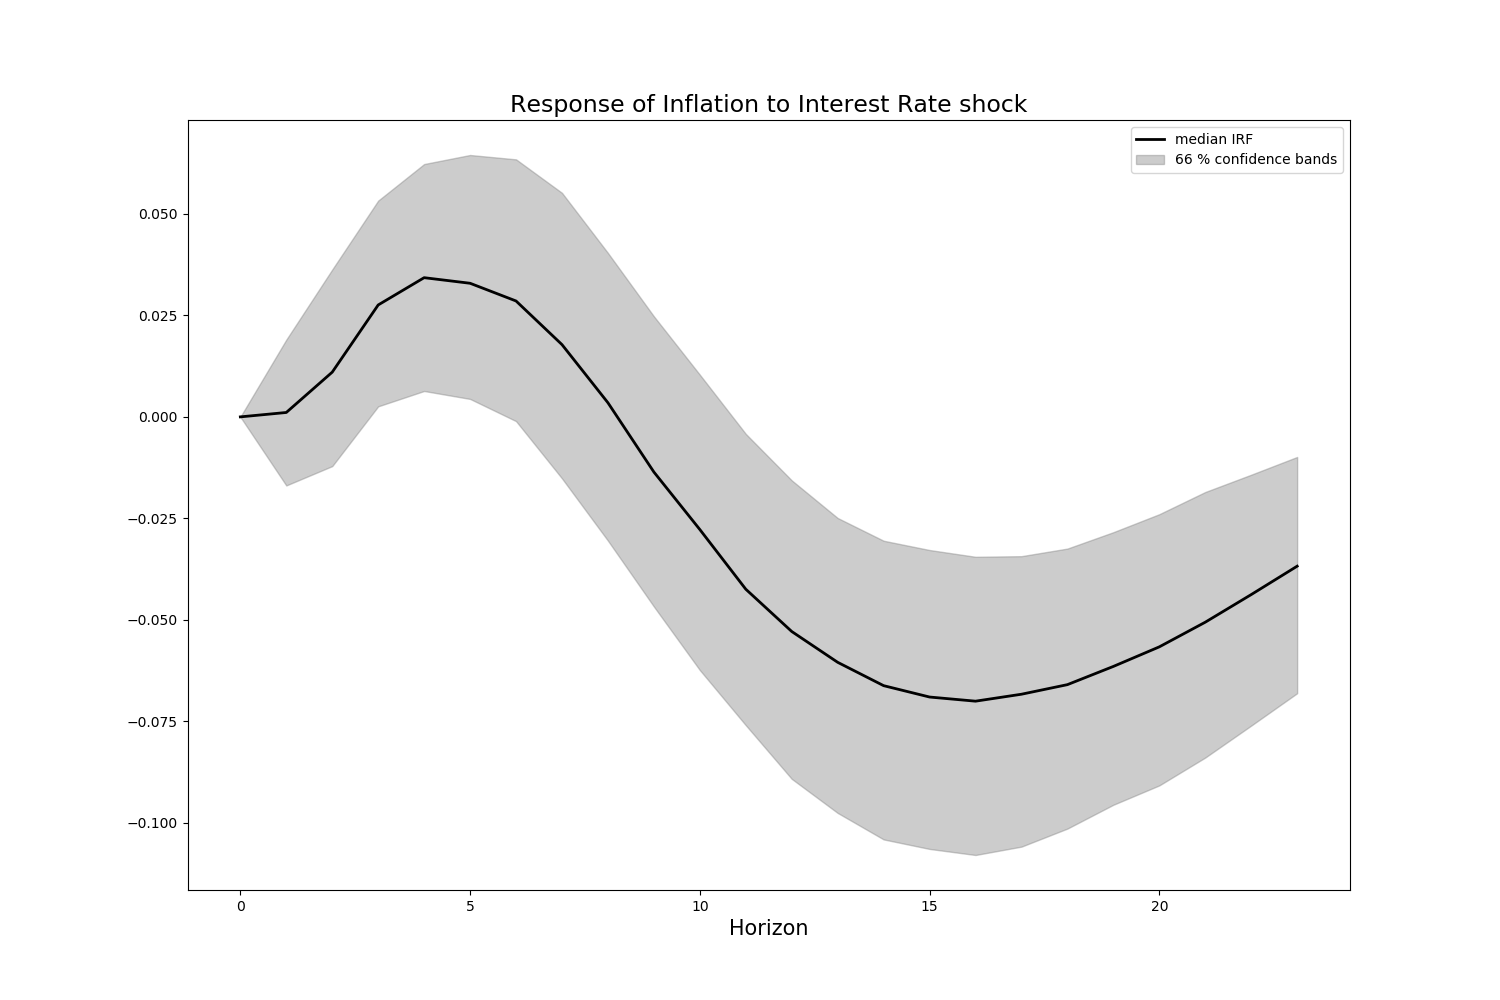
\includegraphics[width=0.7\linewidth]{../replication/VAR/Outdata/IRFs_poor/IRF_rffr_sprice}
			\caption{Response of inflation to interest rate shock.}
			\label{fig:}
		\end{figure}}		
	\only<2>{\begin{figure}
			\centering
			\includegraphics[width=0.7\linewidth]{../replication/VAR/Outdata/IRFs_poor/IRF_rffr_su3}
			\caption{Response of unemployment to interest rate shock.}
			\label{fig:}
		\end{figure}}		
	\only<3>{\begin{figure}
			\centering
			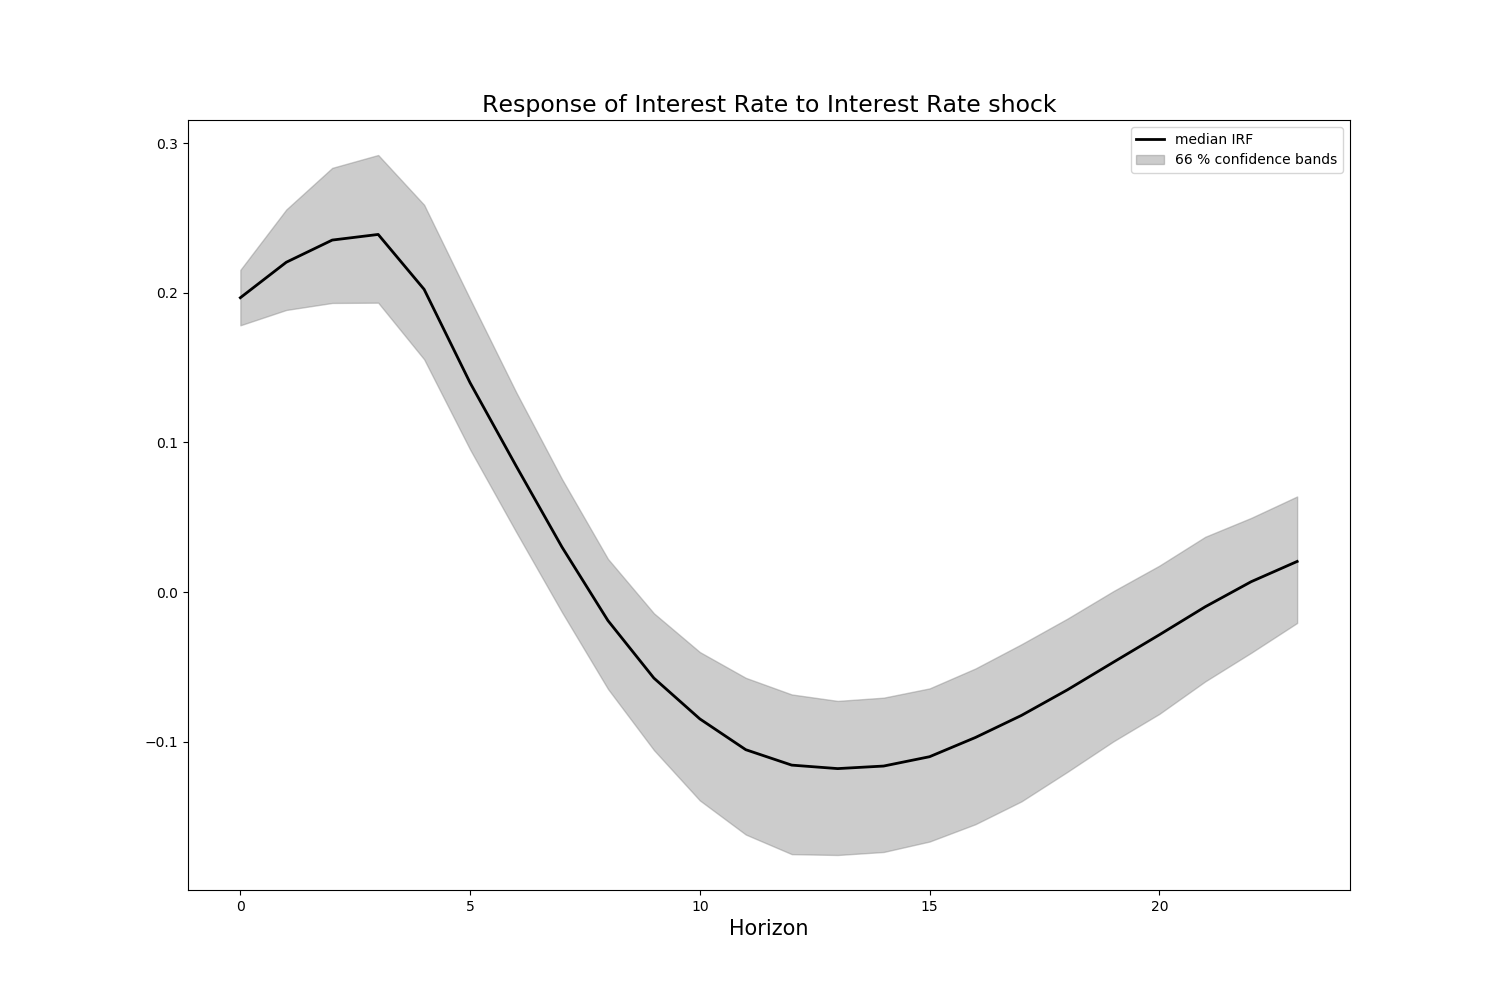
\includegraphics[width=0.7\linewidth]{../replication/VAR/Outdata/IRFs_poor/IRF_rffr_sffr}
			\caption{Response of interest rate to interest rate shock.}
			\label{fig:}
		\end{figure}}		
	\end{frame}
	
	
	\begin{frame}{IRFs: responses to inflation shock}
	\only<1>{\begin{figure}
			\centering
			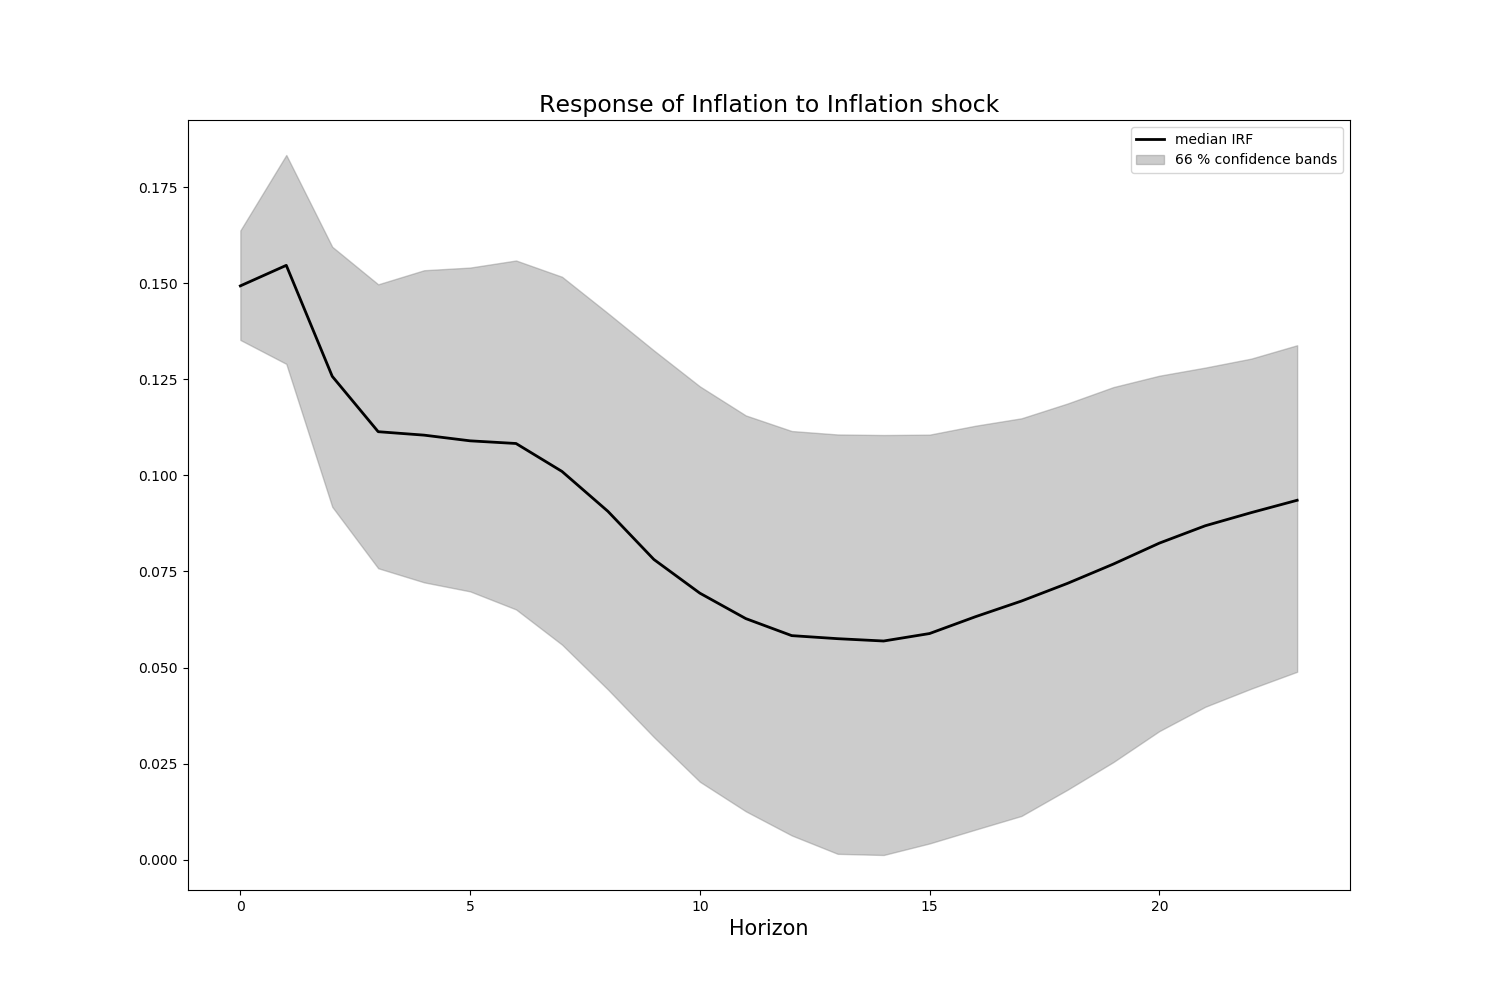
\includegraphics[width=0.7\linewidth]{../replication/VAR/Outdata/IRFs_poor/IRF_rprice_sprice}
			\caption{Response of inflation to inflation shock.}
			\label{fig:}
		\end{figure}}
		\only<2>{\begin{figure}
		\centering
		\includegraphics[width=0.7\linewidth]{../replication/VAR/Outdata/IRFs_poor/IRF_rprice_su3}
		\caption{Response of unemployment to inflation shock.}
		\label{fig:}
		\end{figure}}		
		\only<3>{\begin{figure}
		\centering
		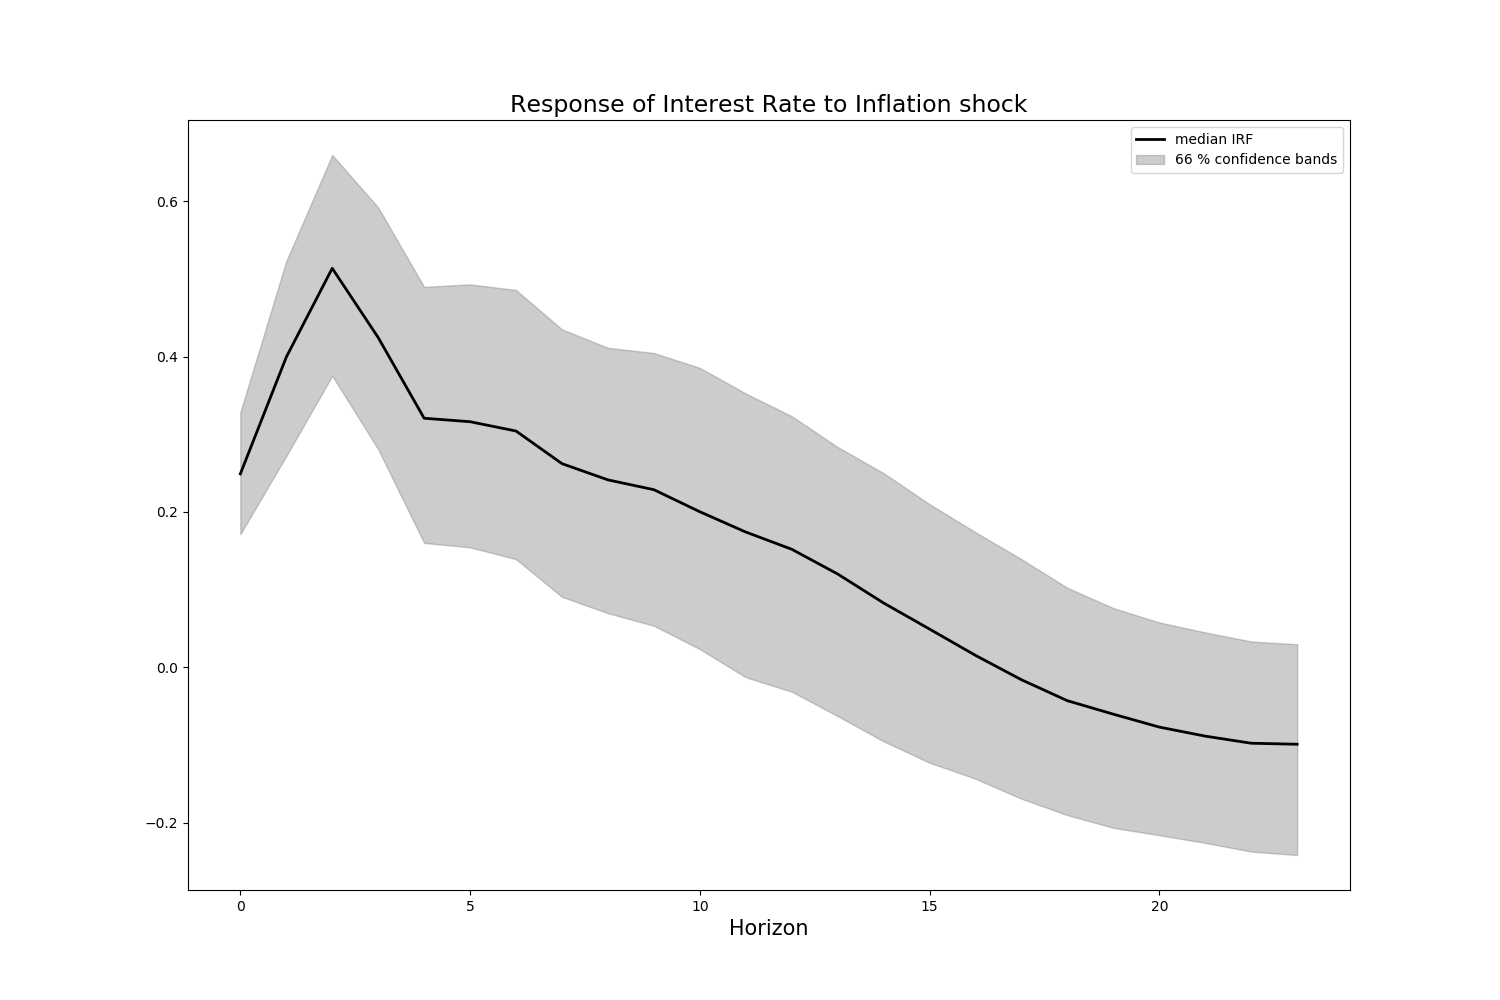
\includegraphics[width=0.7\linewidth]{../replication/VAR/Outdata/IRFs_poor/IRF_rprice_sffr}
		\caption{Response of interest rate to inflation shock.}
		\label{fig:}
		\end{figure}}		
	\end{frame}	

	\begin{frame}{More on VARs}
		\begin{itemize}
			\item More identification techniques (e.g. sign restrictions; partial identification)
			\pause
			\item Including more structure (e.g. Taylor rule)
			\pause
			\item Time-varying parameters (TVARs)
		\end{itemize}
		\vspace*{1em}
		\pause
		How to deal with...
		\pause
		\begin{itemize}
			\item Mixed-frequency data
			\pause
			\item Missing data
			\pause
			\item Jagged-edges data
		\end{itemize}		
	\end{frame}
	

	\begin{frame}{References:}
		\underline{Main:}
		\small{
		\begin{itemize}
			\item Doan, Thomas, et al. “Forecasting and Conditional Projection Using Realistic Prior Distributions.” Econometric Reviews, vol. 3, no. 1, 1984, pp. 1–100.			
			\item Hamilton, James D. ``Time Series Analysis." Princeton University Press, 1994.			
			\item Sims, Christopher A. ``Macroeconomics and Reality." \textit{Econometrica} 48, no. 1 (1980): 1-48.
			\item Stock, James H., and Mark W. Watson. ``Vector Autoregressions." \textit{The Journal of Economic Perspectives} 15, no. 4 (2001): 101-15.
			\item Uhlig, H. ``Economics and Reality." \textit{MFI Working Paper Series} no. 2011-006.			
		\end{itemize}}
	\end{frame}
\end{document}

